\documentclass{article}
\usepackage[T1]{fontenc}
\usepackage{graphicx}
\usepackage{subcaption}
\usepackage{sectsty}
\usepackage{multirow}
\usepackage[a4paper, total={6in, 8in}]{geometry}

\def\v{0.4}

\title{%
	Algorytmy Metahuerystyczne \\
	\large Lista 1}
\author{Szymon Janiak}
\begin{document}
\maketitle

\sectionfont{\centering}
\subsectionfont{\centering}
\section*{Opis problemu}
	Obliczamy wagę minimalnego drzewa rozpinającego, średnią wartość uzyskanego rozwiązania, średnią liczbę kroków poprawy oraz najlepsze uzyskane rozwiązanie dla 3 sposobów z wykorzystaniem algorytmu Local Search
	\begin{enumerate}
	    \item Local Search użyty na cyklu stworzonego z minimalnego drzewa rozpinającego
	    \item Local Search użyty na losowej permutacji
	    \item Local Search użyty na losowej permutacji z wybieraniem najlepszego sąsiada z $n$ losowo wybranych
	\end{enumerate}

\subsection*{Waga uzyskanych najlepszych rozwiązań}
    \begin{center}
    \resizebox{15cm}{!}{
        \begin{tabular}{|c||c|c|c|c|c|}
        \hline
            nic & MST & TSP & $local\_search$ 1  & $local\_search$ 2 &$local\_search$ 3\\
            \hline\hline
            xqf131 & 476 & 756 & 540 & 564 & 574\\
            \hline
            xqg237 & 906 & 1380 & 1097 & 1156 & 1160\\
            \hline
            pma343 & 1183 & 1810 & 1476 & 1524 & 1585\\
            \hline
            pka379 & 1160 & 1851 & 1431 & 1494 & 1461\\
            \hline
            bcl380 & 1453 & 2307 & 1748 & 1775 & 1773\\
            \hline
            pbl395 & 1132 & 1753 & 1374 & 1400 & 1430\\
            \hline
            pbk411 & 1189 & 1793 & 1418 & 1486 & 1492\\
            \hline
            pbn423 & 1210 & 1873 & 1468 & 1537 & 1537\\
            \hline
            pbm436 & 1277 & 1970 & 1529 & 1562 & 1565\\
            \hline
            xql662 & 2249 & 3571 & 2713 & 2805 & 2809\\
            \hline
            xit1083 & 3256 & 4996 & 3834 & 4063 & 4016\\
            \hline
            icw1483 & 4017 & 5927 & 4668 & 5020 & 5112\\
            \hline
            djc1785 & 5550 & 8282 & 6440 & 6749 & 7208 \\
            \hline
            dcb2086 & 5958 & 9186 & 7063 & 7321 & 7476\\
            \hline
            pds2566 & 6964 & 10673 & 8219 & 8611 & 9830 \\
        \hline
		\end{tabular}}
    \end{center}


\begin{table}[h!]
    \centering
    \begin{tabular}{|c|c|c|c|c|c|c|}
        \hline
        \multirow{2}{*}{Przykład} & \multicolumn{2}{|c|}{$local\_search$ 1} & \multicolumn{2}{|c|}{$local\_search$ 2}  & \multicolumn{2}{|c|}{$local\_search$ 3}  \\
        \cline{2-7}
        & \multicolumn{2}{c|}{średnia} & \multicolumn{2}{c|}{średnia} & \multicolumn{2}{c|}{średnia} \\
        \cline{2-4} \cline{4-5} \cline{6-7}
        & liczba popraw & suma wag & liczba popraw & suma wag & liczba popraw & suma wag \\
        \hline
        xqf131 & 28.8 & 701.9 & 62.3 & 712.4 & 51.9 & 722.4 \\
        \hline
        xqg237 & 37.0 & 1483.7 & 130.5 & 1415.8 & 112.2 & 1445.9 \\
        \hline
        pma343 & 75.8 & 1650.3 & 201.9 & 1684.7 & 183.3 & 1717.1 \\
        \hline
        pka379 & 78.9 & 1716.3 & 224.7 & 1745.9 & 204.9 & 1742.7 \\
        \hline
        bcl380 & 62.7 & 1949.3 & 223.7 & 1917.5 & 189.2 & 1913.5 \\
        \hline
        pbl395 & 80.0 & 1771.5 & 227.8 & 1829.0 & 193.4 & 1876.2 \\
        \hline
        pbk411 & 81.6 & 1837.9 & 242.7 & 1888.5 & 203.6 & 2181.15 \\
        \hline
        pbn423 & 72.3 & 1873.9 & 249.0 & 1921.6 & 219.8 & 2081.5 \\
        \hline
        pbm436 & 97.85 & 2562.5 & 256.8 & 2312.0 & 217.4 & 2363.1 \\
        \hline
        xql662 & 122.6 & 3690.4 & 405.4 & 3813.3 & 349.1 & 3917.5 \\
        \hline
        xit1083 & 191.6 & 4312.2 & 693.7 & 4721.2 & 623.9 & 4826.1 \\
        \hline
        icw1483 & 278.8 & 5034.6 & 973.4 & 5301.2 & 834.5 & 5718.2 \\
        \hline
        djc1785 & 382.6 & 6733.8 & 1193.9 & 6872.1 & 1032.6 & 7764.5 \\
        \hline
        dcb2086 & 390.9 & 7454.2 & 2392.6 & 7457.8 & 1222.2 & 8888.3 \\
        \hline
        pds2566 & 457.3 & 8671.4 & 1742.9 & 8701.8 & 1526.0 & 10687.5 \\
        \hline
    \end{tabular}
\end{table}

\subsection*{Wnioski}
	Z wyników można wywnioskować, że rozwiązanie tworzone poprzed $local\_search$ na podstawie MST daje najlepsze wyniki. Do tego widzimy znaczą poprawe względem zwykłego TSP. Testowanie części otoczenia zmniejsza średnią ilość przeprowadzonych popraw, jednak prowadzi do gorszych wyników.

\clearpage

\subsection*{Wizualizacje}
    \begin{figure}[h!]
		\centering
		\begin{subfigure}[b]{\v\linewidth}
			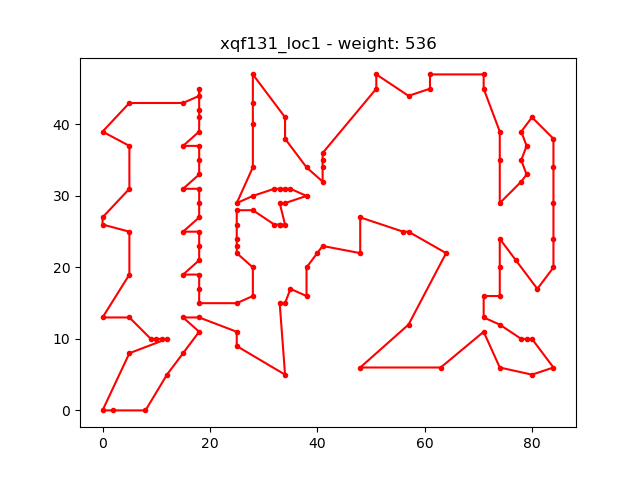
\includegraphics[width=\linewidth]{graphs/TSP_xqf131_loc1.png}
		\end{subfigure}
		\begin{subfigure}[b]{\v\linewidth}
			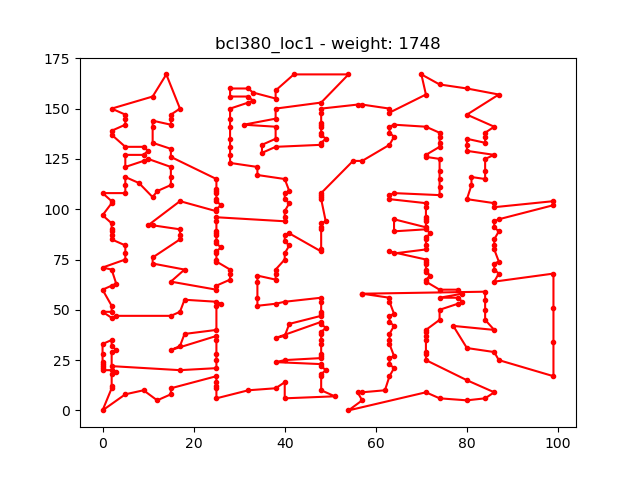
\includegraphics[width=\linewidth]{graphs/TSP_bcl380_loc1.png}
		\end{subfigure}
		\begin{subfigure}[b]{\v\linewidth}
			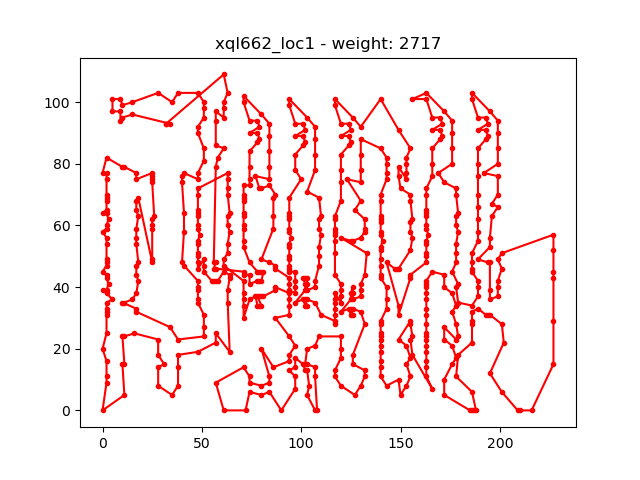
\includegraphics[width=\linewidth]{graphs/TSP_xql662_loc1.png}
		\end{subfigure}
		\begin{subfigure}[b]{\v\linewidth}
			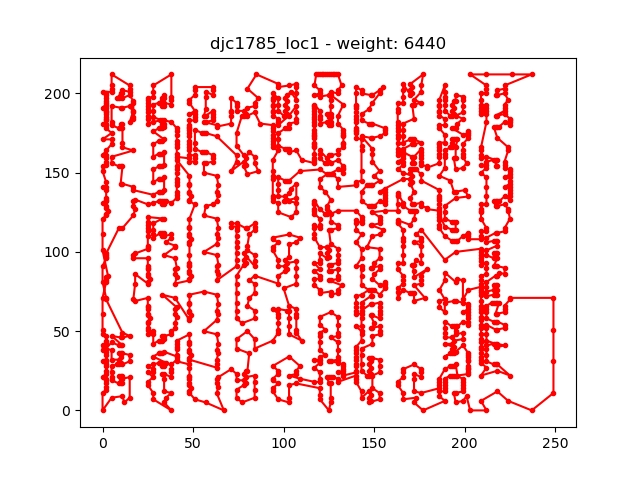
\includegraphics[width=\linewidth]{graphs/TSP_djc1785_loc1.png}
		\end{subfigure}
		\begin{subfigure}[b]{\v\linewidth}
			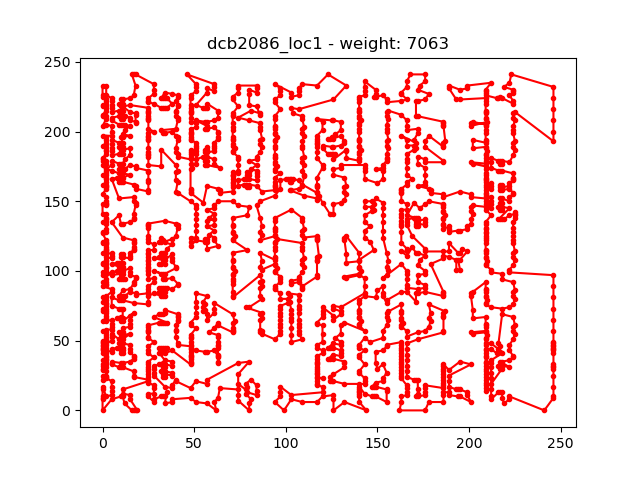
\includegraphics[width=\linewidth]{graphs/TSP_dcb2086_loc1.png}
		\end{subfigure}
		\begin{subfigure}[b]{\v\linewidth}
			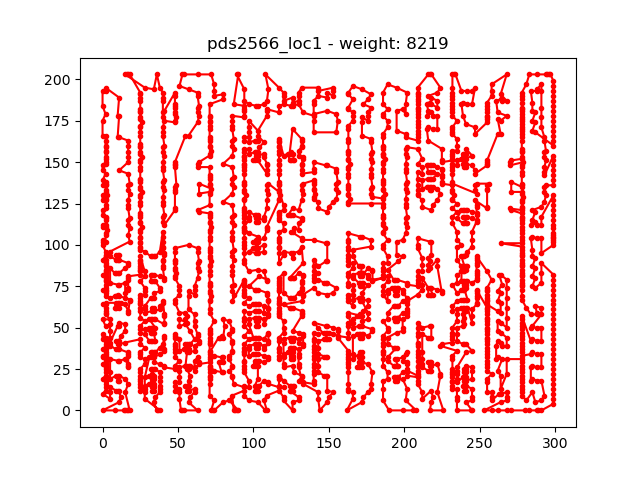
\includegraphics[width=\linewidth]{graphs/TSP_pds2566_loc1.png}
		\end{subfigure}
	\end{figure}

	\begin{figure}[h!]
		\centering
		\begin{subfigure}[b]{\v\linewidth}
			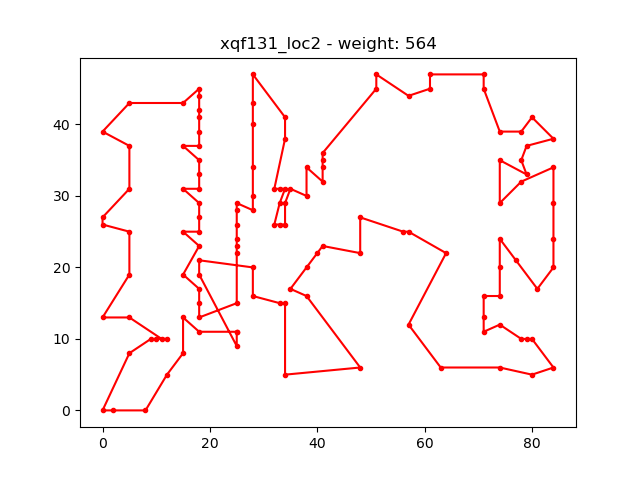
\includegraphics[width=\linewidth]{graphs/TSP_xqf131_loc2.png}
		\end{subfigure}
		\begin{subfigure}[b]{\v\linewidth}
			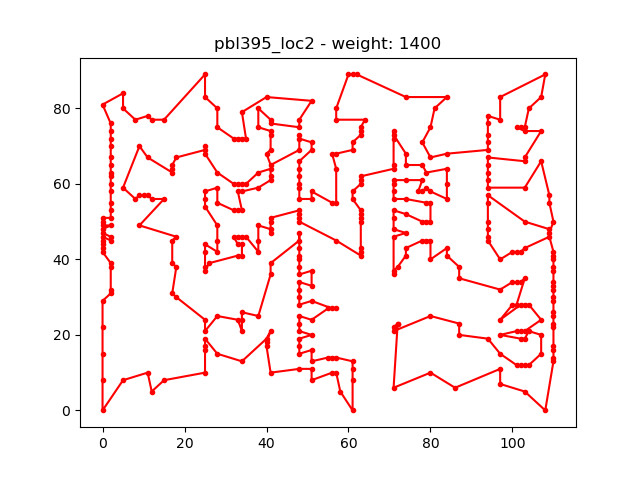
\includegraphics[width=\linewidth]{graphs/TSP_pbl395_loc2.png}
		\end{subfigure}
		\begin{subfigure}[b]{\v\linewidth}
			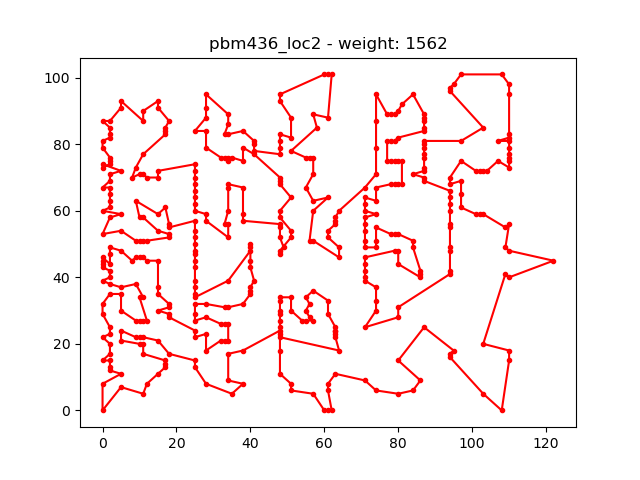
\includegraphics[width=\linewidth]{graphs/TSP_pbm436_loc2.png}
		\end{subfigure}
		\begin{subfigure}[b]{\v\linewidth}
			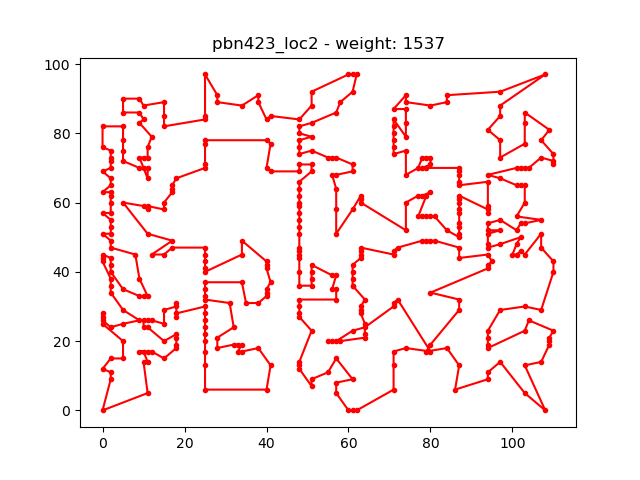
\includegraphics[width=\linewidth]{graphs/TSP_pbn423_loc2.png}
		\end{subfigure}
		\begin{subfigure}[b]{\v\linewidth}
			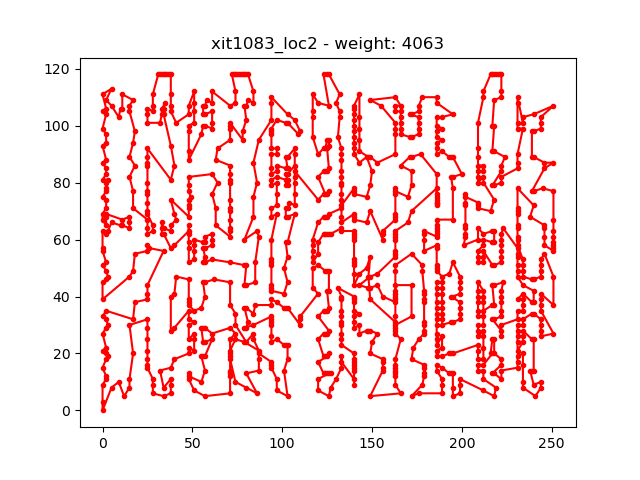
\includegraphics[width=\linewidth]{graphs/TSP_xit1083_loc2.png}
		\end{subfigure}
		\begin{subfigure}[b]{\v\linewidth}
			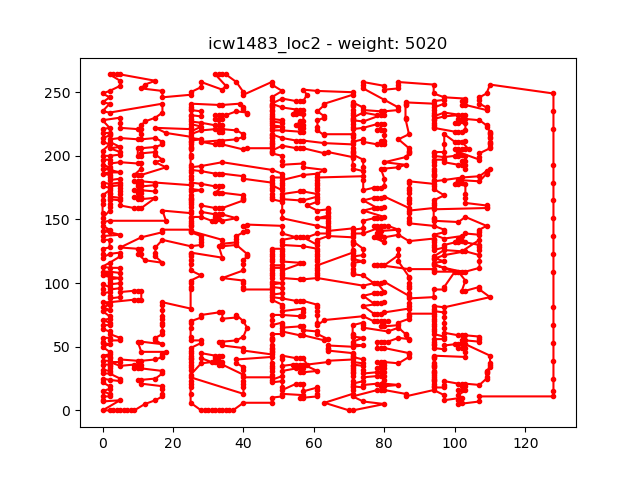
\includegraphics[width=\linewidth]{graphs/TSP_icw1483_loc2.png}
		\end{subfigure}
	\end{figure}

	\begin{figure}[h!]
		\centering
		\begin{subfigure}[b]{\v\linewidth}
			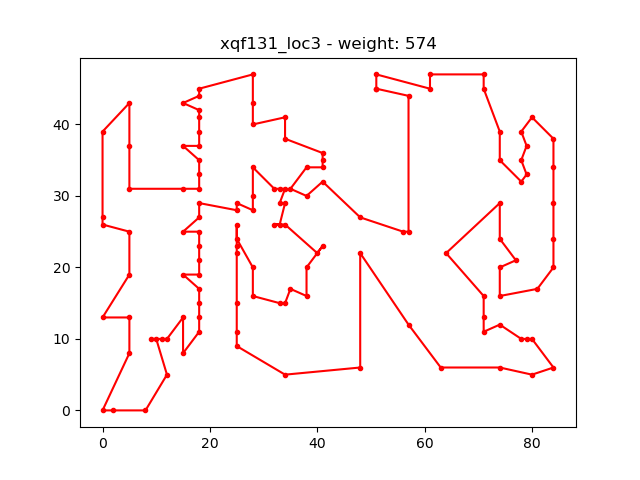
\includegraphics[width=\linewidth]{graphs/TSP_xqf131_loc3.png}
		\end{subfigure}
		\begin{subfigure}[b]{\v\linewidth}
			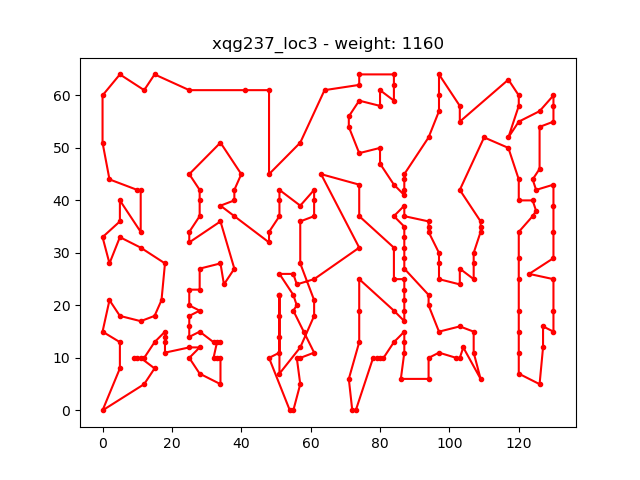
\includegraphics[width=\linewidth]{graphs/TSP_xqg237_loc3.png}
		\end{subfigure}
		\begin{subfigure}[b]{\v\linewidth}
			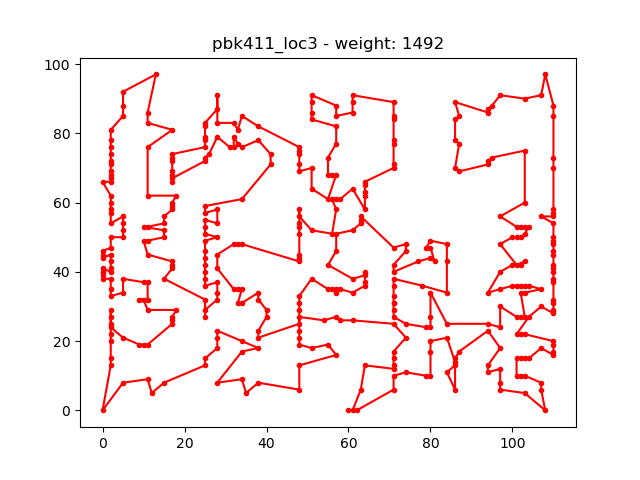
\includegraphics[width=\linewidth]{graphs/TSP_pbk411_loc3.png}
		\end{subfigure}
		\begin{subfigure}[b]{\v\linewidth}
			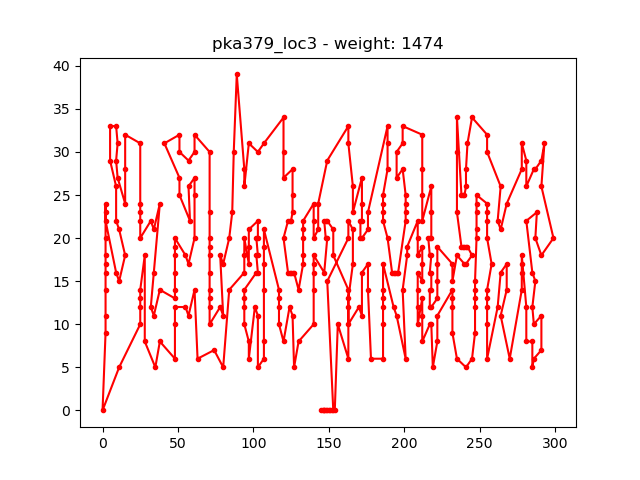
\includegraphics[width=\linewidth]{graphs/TSP_pka379_loc3.png}
		\end{subfigure}
		\begin{subfigure}[b]{\v\linewidth}
			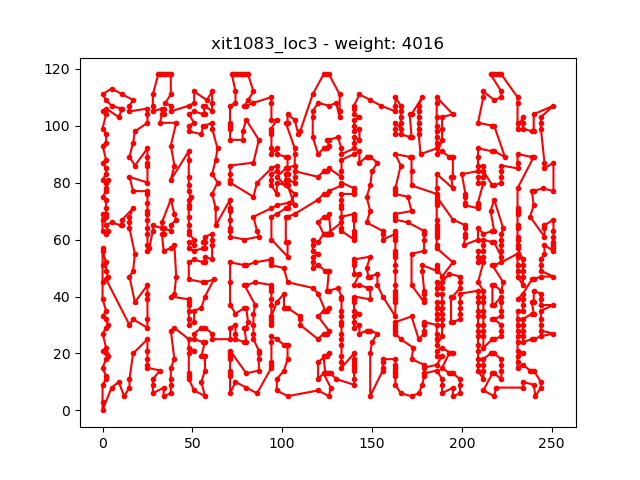
\includegraphics[width=\linewidth]{graphs/TSP_xit1083_loc3.png}
		\end{subfigure}
	\end{figure}
\end{document}